\documentclass[11pt, oneside]{book}
\newcommand{\version}{v1.02}

\usepackage[pdftex,a4paper]{geometry}
\usepackage{pdfpages}
\usepackage{graphicx}
\usepackage{amssymb}
\usepackage{gensymb}
\usepackage{eurosym}
\usepackage{ifthen}
\usepackage{float}
\usepackage{calc}
\usepackage[export]{adjustbox}% http://ctan.org/pkg/adjustbox
\usepackage{xstring}
\usepackage{multicol}
\usepackage[framemethod=TikZ]{mdframed}
\usepackage[T1]{fontenc}

% Switch font comprehensively
\usepackage[scaled]{helvet}
\renewcommand\familydefault{\sfdefault} 

% Use as much of the page as we can.
\pagestyle{empty}
\setlength{\parindent}{4em}
\setlength{\parskip}{1.2em}
\setlength{\textheight}{28cm}
\setlength{\textwidth}{19cm}
\setlength{\hoffset}{-2cm}
\setlength{\voffset}{-2cm}

% DECAL function
%
% The decal function takes 5 inputs and extracts a symbol from the Italian ISO document that is included in this repository. The function then displays the symbol together with the title and warning text.
%
% Parameters:		#1 Page with the symbol on it in the document.
%			#2 Title
%			#3 Y height on the page.
%			#4 X location on the page. (not sure on this)
%			#5 Warning subtext
%
\newcommand{\decal}[5]{
\begin{minipage}{\linewidth}
	\begin{minipage}[t]{0.3\textwidth}
	       \vspace{0pt}
	       % The ISO document has a 'gutter' - so we shift the X a bit on the left/right page.
	       %
		\ifthenelse{\isodd{#1}}{ %if the pagenumber is odd, use this location for the image
			\includegraphics[width=0.9\textwidth,page=#1,viewport=103 #3 291 #4,clip=true]{13GR_PistopioimeniSimansi_ISO_7010.pdf}
		}{ %else (because the pagenumber is even), use this location for the image.
			\includegraphics[width=0.9\textwidth,page=#1,viewport=70 #3 261 #4,clip=true]{13GR_PistopioimeniSimansi_ISO_7010.pdf}
		}
	\end{minipage}
	\begin{minipage}[t]{0.6\textwidth}
		\setlength{\parindent}{4em}
		\setlength{\parskip}{1.2em}
	       \vspace{0pt}\raggedright
		{\LARGE \textbf{#2}} %include title text in bold and such
	
		#5 %include warning subtext
		\vspace{0.5cm}
	\end{minipage}
\end{minipage}
}


% Some home made symbols which are not part of the official ISO list of symbols:
%
% Two person symbol
\newcommand{\twopersons}{
\raisebox{-.5\height}{\includegraphics[width=6mm]{File:Aiga_toiletsq_men}}\textbf{x 2} 
}

% Some home made symbols which are not part of the official ISO list of symbols:
% Clock with 7-19 symbol
%
\newcommand{\seventoseven}{
\raisebox{-.5\height}{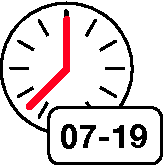
\includegraphics[width=10mm]{clock-limits}}
}


% Define classes for Action, Prohibit and Warn. These each take three inputs.
%
% Turns out that the symbols extracted from the ISO document with \decal are a bit 
% shifted in the Y position or size depending on what class they are. So we split
% them into the three sections that have height differences.
%
% Parameters:		Page with the symbol on it. Actual pagenumber, not the number on the page!
%			Title
%			Warning subtext
%
\newcommand{\action}[3]{\decal{#1}{#2}{520}{715}{#3}}
\newcommand{\prohib}[3]{\decal{#1}{#2}{495}{690}{#3}}
\newcommand{\warn}[3]{\decal{#1}{#2}{520}{715}{#3}}

%% Command to create a round box to call extra attention to something.
%%
\newcommand{\smallicontext}[2]{%
\begin{mdframed}[roundcorner=4pt] 
\begin{tabular}{lp{0.8\linewidth}}
#1 & #2 \\
\end{tabular}
\end{mdframed}
}

% machinePage
% A full page with a machine on it. Takes 5 inputs.
%
% Params:		#1 Machine name
%			#2 Tokens for standard instrutions: Zero or more from
%				Approval	Trustee approval needed.
%				Noise		Not after 19:00
%				Two		Two people required
%				Log		use must be logged
%				Dewalt		Attach dewalt dutch extractor.
%			#3 Specific instructions - added to the above text.
%			#4 Warnings, Symbols - main symbols on page.
%			#5 Extra footer/bottom of the page text
%
\newcommand{\machinePage}[5]{%
\begin{center}
	\vspace{0cm}
	{\fontsize{50}{60} \textbf{#1}}%Machine name
 
	\action{49}{% Determines if you require approval / mandatory instructions / safety instructions
		\textbf{%
 		\IfSubStr{#2}{Approval}%
			{Instructions \& Approval Mandatory}
			{\IfSubStr{#2}{NoMandatory}{Mandatory Safety Rules}{Instruction Mandatory}}%
		}}
		{%
		\IfSubStr{#2}{NoMandatory}{}{Instruction \textbf{prior} to use is \textbf{mandatory}. Check the wiki for who can help you.}
		\IfSubStr{#2}{Approval}{You must also have a `\textbf{dangerous equipment waiver}' filed with the foundations trustees and been given \textbf{approval or card access} to use the machine.}{}
			
		#3 % added to above instructions
		
		\IfSubStr{#2}{Noise}{\smallicontext{\seventoseven}{
			Machine can only be used between 07:00 - 19:00 (be kind to our neighbours)
			}
		}{}

		\IfSubStr{#2}{Two}{\smallicontext{\twopersons}{A second person must be present during operation, have agreed to be your second, knows how to stop the machine and what to do in an emergency, including opening the door for paramedics if needed.	}
		}{}

		\IfSubStr{#2}{Log}{Report any use in the log - and \textbf{pay for it}!}{}

		\IfSubStr{#2}{Dewalt}{Be sure to attach and power on the dust extractor.}{}
	}
	\begin{multicols}{2}#4\end{multicols}
	
	\vspace{0.2cm}
	#5
%footer text at the bottom of the page.
	If a machine is not clean or appears broken - then report this to the mailing list. Clean/fix prior to use.

	\textbf{Report any damage, issues or accident within 24 hours to the mailing list.}
\end{center}
\vfill
\begin{flushright}
{\tiny \version -- \today}
\end{flushright}
\pagebreak
}







\begin{document}
%: Intro
\machinePage{Makerspace}{NoMandatory}{
Observe all safety instructions. Instructions or approval is required for some of the machines. Ask someone for help, consult the wiki or email the mailing lists when in doubt.

Ask for instructions if you are unfamiliar on how to use a tool. This is to protect you and to protect the tool. This is a shared space -- consider others around you before using a machine; and be aware of others working nearby.  Leave the space cleaner than you found it.

Make sure you know where the \textbf{emergency stops and fire extinguishers} are. In case of "call 112"-type emergencies, make sure there is someone at the door to let paramedics in. If you have to stay with the wounded, jam the doors open. Bring your key(card)s with you if you have to let emergency personnel in.
}{
\action{58}{Wear protective clothing}{Wear tight fitting clothing, keep long hair out tied up, no jewellery or anything else that can be caught by a machine. Consider that others may be working at the space -- and you may be in close range of their machines too.

%Be careful with gloves -- they can be caught in the machine and when made of a sturdy material, help rip your finger off. Observe the `no gloves' signs.
}
\action{56}{Wear appropriate footwear}{No sandals or similar in the main workspace.}
\action{64}{Wear a mask when needed}{Especially when cutting materials such as MDF}
\action{52}{Eye protection recommended}{Also consider that hard-metal cutters and ceramics can suddenly shatter.}
\action{57}{Protective gloves recommended}{But also: be careful with gloves -- they can be caught in the machine and when made of a sturdy material, help rip your finger off. }
\action{51}{Ear protection recommended}{And try to be considerate Neighbours--especially after 19:00.}
}{If something breaks or is amiss -- it is \textbf{your} responsibility to report it.  If you find something broken -- report it before using/repairing the machine.
}

%%%%%%%%%%%%%%%%%%%%%%%%%%%%%%%%%%%%%%%%%%
%: Arboga G2508 Pillar Drill
\machinePage{Arboga G2508 Pillar Drill}{noise}{
\textbf Use proper drill speed. (See table)}{


\prohib{100}{Do not wear gloves}{Especially strong leather ones. They get caught easily and then `help' ripping body parts off.}

\action{52}{Eye protection recommended}{Swarf will fly. Marterial can come loose.}
\action{58}{Wear protective clothing}{Wear tight fitting clothing, keep long hair out tied up, no jewellery or anything else that can be caught by the machine.}
	
\warn{130}{Crushing}{Risk of crushing -- the machine does not have any sensors that detect obstacles. The drill is operated by gears. They will no slip or stop.
This includes things such as your hands or tools you've left on the workspace.}
}{
Noise wise -- be considerate to our neighbours -- especially in the evenings.}

%%%%%%%%%%%%%%%%%%%%%%%%%%%%%%%%%%%%%%%%%%
%: Large CNC Cutter
\machinePage{Large CNC Cutter}{Noise}{
}{
\action{51}{Ear protection strongly recommended}{Note also that this machine should not be used after 19:00}
\action{52}{Eye protection recommended}{Especially when using very small cutters.}
\action{64}{Wear a mask when needed}{Especially when cutting materials such as MDF}

\warn{130}{Crushing}{Risk of crushing -- the machine does not have any sensors that detect obstacles
This includes things such as your hands (do not lean on the blue rail) or tools you've left on the workspace.
}
}

%%%%%%%%%%%%%%%%%%%%%%%%%%%%%%%%%%%%%%%%%%
%: Abene
\machinePage{Abene Mill}{Approval}{
}{
\prohib{100}{Do not wear gloves}{Especially strong leather ones. They get caught easily and then `help' ripping body parts off.}
\action{52}{Eye protection recommended}{Swarf will fly. Cutters can come loose. Broken cutters can fly very far and are razor sharp.}
\action{58}{Wear protective clothing}{Wear tight fitting clothing, keep long hair out tied up, no jewellery or anything else that can be caught by the machine.}
\warn{125}{Crushing}{Risk of crushing -- the machine does not have any sensors that detect obstacles.

Note that it can also run very slow; barely noticeable.}
\warn{117}{Slippery surface}{Floor will get very slippery; especially when using coolant.}
\warn{128}{Sharp rotating elements}{This machine is essentially a cutter without any guard whatsoever.}
}{
Only switch XYZ feeds when the machine is not running. Use the hand-wheel to get the gear fully locked in prior to starting the feed. Be sure to tighten all 4 nuts post rotating the head or all 4 nuts when moving the head laterally.

Try to avoid getting coolant or similar on the slide-ways -- especially the Y slipway between machine and table. Use a shield or adjust the flow. Machine needs to be cleaned post use.  When using coolant -- also empty the recess on the left of the table and clean out the t-Slots until dry.
}

%%%%%%%%%%%%%%%%%%%%%%%%%%%%%%%%%%%%%%%%%%
%: Metal Lathe
\machinePage{Metal Lathe}{Approval}{
Be careful when using the auto-feed; especially with cutters near the revolving head.
}{
\prohib{100}{Do not wear gloves}{Especially strong leather ones. They get caught easily and then `help' ripping body parts off.}
\action{52}{Eye protection recommended}{Swarf will fly. Cutters can come loose. Broken cutters can fly very far and are razor sharp.}
\action{58}{Wear protective clothing}{Wear tight fitting clothing, keep long hair out tied up, no jewellery or anything else that can be caught by the machine.}
\warn{125}{Crushing}{Risk of crushing -- the machine does not have any sensors that detect obstacles.

Note that it can also run very slow; barely noticeable.}
\warn{117}{Slippery surface}{Floor may get slippery when using coolant.}
% \warn{128}{Sharp rotating elements}{This machine is essentially a cutter without any guard whatsoever.}
}{
Clean after use -- especially when you have used coolant or have used metals that can rust easily or cause a galvanic reaction.
}
%%%%%%%%%%%%%%%%%%%%%%%%%%%%%%%%%%%%%%%%%%
%: Wood Lathe
\machinePage{Wood Lathe}{Approval}{
This machine is for WOOD only.
}{
\action{64}{Wear a mask when needed}{Especially when cutting materials such as MDF}
\action{58}{Wear protective clothing}{Wear tight fitting clothing, keep long hair out tied up, no jewellery or anything else that can be caught by the machine.}
\action{52}{Eye protection mandatory}{}
\prohib{100}{Not recommended to wear gloves}{}
}{
}

%%%%%%%%%%%%%%%%%%%%%%%%%%%%%%%%%%%%%%%%%%
%: Afkortzaag
\machinePage{Mitre saw}{Noise}{
This machine is for WOOD only.

}{
\action{58}{Wear protective clothing}{Wear tight fitting clothing, keep long hair out tied up, no jewellery or anything else that can be caught by the machine.}
\action{52}{Eye protection recommended}{}
\action{51}{Ear protection recommended}{Note also that this machine should not be used after 19:00 if it is that noisy}
\action{64}{Wear a mask when needed}{Especially when cutting materials such as MDF}
\warn{128}{Sharp rotating elements}{So keep your fingers away. Bypassing or using your fingers to hold the guard open is downright stupid.}
}{}

%%%%%%%%%%%%%%%%%%%%%%%%%%%%%%%%%%%%%%%%%%
%: Circelzaag
\machinePage{Wood Circle-saw Table}{Approval,Noise,Two,Dewalt}{
This machine is for WOOD only.
}{
\action{51}{Ear protection strongly recommended}{Note also that this machine should not be used after 19:00}
\action{58}{Wear protective clothing}{Wear tight fitting clothing, keep long hair out tied up, no jewellery or anything else that can be caught by the machine.}
\action{52}{Eye protection recommended}{Especially when using very small cutters.}
\action{64}{Wear a mask when needed}{Especially when cutting materials such as MDF}
\prohib{100}{Do not wear gloves}{Especially strong leather ones. They get caught easily and then `help' ripping body parts off.}
}{
}

%%%%%%%%%%%%%%%%%%%%%%%%%%%%%%%%%%%%%%%%%%
%: Lintzaag
\machinePage{Wood Bandsaw}{Approval,Dewalt}{
This machine is for WOOD only.
}{
\action{51}{Ear protection strongly recommended}{Note also that this machine should not be used after 19:00}
\action{58}{Wear protective clothing}{Wear tight fitting clothing, keep long hair out tied up, no jewellery or anything else that can be caught by the machine.}
\action{52}{Eye protection recommended}{}
\action{64}{Wear a mask when needed}{Especially when cutting materials such as MDF}
}{
}

%%%%%%%%%%%%%%%%%%%%%%%%%%%%%%%%%%%%%%%%%%
%: Planer
\machinePage{Planer}{Approval, Noise, Two}{
This machine is for WOOD only.
}{
\warn{131}{Counterrotating rollers}{This machine will `pull' you in using counter rotating rollers. Which ALSO have a ratchet mechanism.}
\action{51}{Ear protection strongly recommended}{Note also that this machine should not be used after 19:00}
\action{58}{Wear protective clothing}{Wear tight fitting clothing, keep long hair out tied up, no jewellery or anything else that can be caught by the machine.}
\action{52}{Eye protection recommended}{}
\action{64}{Wear a mask when needed}{Especially when cutting materials such as MDF}
\prohib{100}{Do not wear gloves}{Especially strong leather ones. They get caught easily and then `help' ripping body parts off.}
}{
}

%%%%%%%%%%%%%%%%%%%%%%%%%%%%%%%%%%%%%%%%%%
%: Jointer
\machinePage{Jointer}{Approval, Noise, Two,Dewalt}{
}{
\warn{128}{Sharp rotating elements}{This machine is essentially a cutter without any guard whatsoever.}
\action{51}{Ear protection strongly recommended}{Note also that this machine should not be used after 19:00}
\action{58}{Wear protective clothing}{Wear tight fitting clothing, keep long hair out tied up, no jewellery or anything else that can be caught by the machine.}
\action{52}{Eye protection recommended}{}
\action{64}{Wear a mask when needed}{Especially when cutting materials such as MDF}
\prohib{100}{Do not wear gloves}{Especially strong leather ones. They get caught easily and then `help' ripping body parts off.}
}{
}

%%%%%%%%%%%%%%%%%%%%%%%%%%%%%%%%%%%%%%%%%%
%: Grote Laser
\machinePage{Large CNC Laser cutter}{Logbook}{
Be sure to check that cooling, air assist and fume extraction fan are all on.
}{
\warn{84}{Do not extinguish with water}{It has a high voltage (kV) power supply. Use the $CO_2$ extinguisher (on the pilar to your left). }
\warn{110}{Laser beam}{Keep the lid closed at all times. If you bypass the safety interlocks -- you are an idiot.}
}{
Do not forget to switch on (and off post use) the compressor and fume extraction fan (in the corner near the electric distribution board.
}
\action{80}{Do not use a forklift in this area}{}
\action{98}{Do not use this CNC laser cutter as a bathtub}{}

%%%%%%%%%%%%%%%%%%%%%%%%%%%%%%%%%%%%%%%%%%
%: Kleine Laser
\machinePage{Small CNC Laser cutter}{Extraction}{
Be sure to check that water cooling pump, air pump (behind the machine) and fume extraction fan are all on.
}{
\warn{84}{Do not extinguish with water}{It has a high voltage (kV) power supply. Use the $CO_2$ extinguisher (on the pilar to your left).}
\warn{110}{Laser beam}{Keep the lid closed at all times. If you bypass the safety interlocks -- you are an idiot.}
}{
Do not forget to switch the fume extraction fan (in the corner near the electric distribution board) post use.
}

%%%%%%%%%%%%%%%%%%%%%%%%%%%%%%%%%%%%%%%%%%
%: Slijpsteen
\machinePage{Large Grinder}{}{
Noise wise -- be considerate to our neighbours -- especially in the evenings.
}{
\action{58}{Wear protective clothing}{Wear tight fitting clothing, keep long hair out tied up, no jewellery or anything else that can be caught by the machine.}
\action{52}{Eye protection needed}{}
\action{51}{Ear protection recommended}{}
}{}

%%%%%%%%%%%%%%%%%%%%%%%%%%%%%%%%%%%%%%%%%%
%: 12 ton press
\machinePage{Hydraulic Press}{}{
}{
\action{52}{Eye protection needed}{}}{
}

%%%%%%%%%%%%%%%%%%%%%%%%%%%%%%%%%%%%%%%%%%
%  Zandstraalcabine
\machinePage{Sanding Cabinet}{}{
Do not spray at your hands/fingers. The gloves \textbf{will} ultimately give way and they are not cheap.
}{
}{
Do switch off the compressor after use.
}

%%%%%%%%%%%%%%%%%%%%%%%%%%%%%%%%%%%%%%%%%%
%: Metaal zaag
\machinePage{Metal bandsaw}{}{
Use plenty of cutting oil, \textsc{wd40} or similar. 

Do not leave unattended (not in the least as you may want to keep lubricating it to get a nice cut).
}{
\action{58}{Wear protective clothing}{Wear tight fitting clothing, keep long hair out tied up, no jewellery or anything else that can be caught by the machine.}
\warn{128}{Sharp rotating elements}{}
\action{52}{Eye protection recommended}{}
}{
}

%%%%%%%%%%%%%%%%%%%%%%%%%%%%%%%%%%%%%%%%%%
%: CNC Vinyl snijder
\machinePage{CNC Vinyl cutter}{}{
}{
\warn{128}{Sharp rotating elements}{}
\warn{124}{Machine can suddenly start}{Also during power-up.}
}{
}

%%%%%%%%%%%%%%%%%%%%%%%%%%%%%%%%%%%%%%%%%%
%:  Reflow oven
\machinePage{PCB Reflow Oven}{}{
}{
}{
}

%%%%%%%%%%%%%%%%%%%%%%%%%%%%%%%%%%%%%%%%%%
%:  Hot plate
\machinePage{T-Shirt hotplate}{}{
}{
\warn{123}{Hot surfaces}{The hotplate will become hot (obviously).}
}{
}

%%%%%%%%%%%%%%%%%%%%%%%%%%%%%%%%%%%%%%%%%%
%:  Welding kit and gas
\machinePage{Welding equipment}{Log}{
Gas cylinders must be kept mounted in their stand with a \textbf{safety strap} at all times.

There should never be more than a total125L of `water equivalent' volume, aggregated across all bottles (full or empty) at the space.
}{
\action{67}{Wear a welding mask}{}
\action{57}{Wear protective gloves}{}
\warn{128}{Pressurised Cylinders}{}
\action{74}{Use protective apron}{}
}{
Do not forget to close the valves on the gas bottles post use.

If you have empty bottles; be sure to get them refilled or remove them from the space. 

There should \textbf{never be more than a 125 litres} of `water equivalent' volume present at the space (aggregated across all cylinders, \textbf{empty or full}, pressured or unpressured).

This is because the space does \textbf{not have the required permits} for crossing the \textbf{125L limit}.
}
%%%%%%%%%%%%%%%%%%%%%%%%%%%%%%%%%%%%%%%%%%
%:   Ultimakers
\machinePage{Ultimaker 2 \& 2$^{+\mathsf{Extended}}$}{}{
Do not walk away from the machine until the first 10 layers or so have been deposited. 

OK to leave unattended after first 10 minutes when used with normal settings/materials.
}{
\warn{124}{Automatic start-up}{Machine may suddenly start moving. Also during power up.}
\warn{123}{Hot surfaces}{The bed and the head will become (very) hot.}
}{
Keep the filament in a sealed container. Exposure to air (humidity) makes it brittle.
}

%:   Drill press
\machinePage{Drill press}{NoMandatory}{
Make sure you clamp your workpiece well - to avoid spinning.

Let the drill do its work - do not apply much pressure (drill gets dull or will snaps).

Use the correct drill speed (higher for aluminium, low for steel, very low for stainless steel (\textsc{rvs}). Use the table on the wall.

Use drilling oil when needed (when in doubt - always use the green oil).
}{
\action{52}{Eye protection recommended}{Sharp bits will fly, drills snap.}
\action{58}{Wear protective clothing}{Wear tight fitting clothing, keep long hair out tied up, no jewellery or anything else that can be caught by the machine.}
\action{57}{Wear protective gloves}{}
\prohib{100}{Wearing gloves not always good}{Wearing gloves can be a mixed blessing - if they are caught in something rotating they may pull your hand towards the machine.}
}{
Noise wise -- be considerate to our neighbours -- especially in the evenings.
}

\machinePage{Hembrug Drill press}{Mandatory}{
Make sure you clamp your workpiece well - to avoid spinning.

Let the drill do its work - do not apply much pressure (drill gets dull or will snaps).

Use the correct drill speed (higher for aluminium, low for steel, very low for stainless steel (\textsc{rvs}). Use the table on the wall.

Use drilling oil when needed (when in doubt - always use the green oil).
}{
\action{52}{Eye protection recommended}{Sharp bits will fly, drills snap.}
\action{58}{Wear protective clothing}{Wear tight fitting clothing, keep long hair out tied up, no jewellery or anything else that can be caught by the machine.}
\prohib{100}{Wearing gloves is forbidden}{Especially strong leather ones. They get caught easily and then `help' ripping body parts off. 
}}
{
\textbf{Beware that this is a powerful, 3-phase (Krachtstroom), machine.}

So unlike the other pillar-drill - it won't stop of something jams.

Beware that the machine can start to spin if you press the green button while the rotary knob is set to 1 or 2. 

Only use the emergency button on the front for emergency stops. For routine on-off use the rotary knob. De-energise the machine with the red button when you are done.

Noise wise -- be considerate to our neighbours -- especially in the evenings.
}


%:   Pottery oven
\machinePage{Pottery Oven}{Mandatory}{
This oven is for pottery, ceramics, annealing and similar use. Up to 1200\degree C.

Please write down the electricity use (kWh counter) and pay \euro{0.25} to the foundation (NL30 TRIO 0197 6945 19).
}{
\prohib{75}{No mid-bake opening}{This oven is not designed to be opened while hot. Or to have contents removed (or added) while hot.}
\prohib{75}{No fumes}{This oven has no exhaust. So no metal melting or similar.}
\warn{118}{Bare electric wires inside}{Do not open the oven while powered on. The heating spirals are not isolated.}
}{
Stay with the machine while it is powered.
}

%: Drill & Mill
\machinePage{Drill \& Mill}{NoMandatory}{
\textbf{Drilling}: Use with common sense, do not drill in the metal of the XY table! Use the wooden overlay to protect it. 

\textbf{Milling}: Getting instructions \textbf{prior} to use is mandatory. After milling: put the machine back in order for drilling, so others can use it

\textbf{When changing the drillbit for milling: use a nylon hamerhead, do NOT use a metal hamer.  }
}{
\prohib{100}{Do not wear gloves}{Especially strong leather ones. They get caught easily and then `help' ripping body parts off. 

Very thin (latex) gloves that easily tear are ok.}
\action{52}{Eye protection recommended}{Especially when milling. Swarf will fly. Cutters can come loose. Broken cutters can fly very far and are razor sharp.}
\action{58}{Wear protective clothing}{Wear tight fitting clothing, keep long hair out tied up, no jewellery or anything else that can be caught by the machine.}
\warn{128}{Sharp rotating elements}{This machine is essentially a cutter without any guard whatsoever.}
\warn{117}{Slippery surface}{Floor will get very slippery; especially when using coolant.}
}{
To adjust the height: 1) loosen the lower nut at the right back side of the machine (marked: 'deze moer' ). Then 2) use the big handle on the left side to crank up/lower the whole top part of the drill. \\
\textbf{And 3) fasten the nut again before drilling!}

For speed adjustment open the top and re-arrange the belts as shown on the diagram on the machine for the right speed. You can run these off/on the wheels by starting and ending with the larger of the two.
}


%: Metal Sander
\machinePage{Metal Sander}{Noise}{
This machine is for metal sanding - both ferrous and non-ferrous metals are allowed (until further notice).

\textbf{Connect a shopvac/vacuum cleaner to keep the dust under control.}

}{
\action{58}{Wear protective clothing}{Wear tight fitting clothing, keep long hair out tied up, no jewellery or anything else that can be caught by the machine.}
\action{51}{Ear protection recommended}{Note also that this machine should not be used after 19:00 -- it is that noisy!}
\action{52}{Eye protection recommended}{}
\action{64}{Wear a mask when needed}{And keep the dust under control by connecting the vacuum cleaner or a shop vac. The grit is both unhealthy \& damaging to other equipment.}
\warn{128}{High speed abrasive surfaces}{So keep your fingers away.  

It takes metal away awfully fast.}{}
}
{Consult the WIKI (or ask) when you need to change the sanding belt. Report this on the mailing list.

Try to leave the machine in at least as clean a state as you found it. Likewise, if you `gum up' the sanding belt (easy with for example soft aluminium) -- do feel encouraged to replace it or at least warn the next user via the mailing list.
}

\machinePage{Wood Router}{Noise}{
This machine is for WOOD only.
}{
\action{58}{Wear protective clothing}{Wear tight fitting clothing, keep long hair out tied up, no jewellery or anything else that can be caught by the machine.}
\action{52}{Eye protection recommended}{}
\action{51}{Ear protection recommended}{Note also that this machine should not be used after 19:00 if it is that noisy}
\action{64}{Wear a mask when needed}{Especially when cutting materials such as MDF}
\warn{128}{Sharp rotating elements}{Bypassing or using your fingers to hold the guard open is downright stupid.}
}{}


%:   Drill press
\machinePage{Oscillating Band/Bobbin Sander}{NoMandatory}{
This machine is for WOOD only.

Make sure that the bobbin/band is fixed in position and cannot slip. 

Let the sander do its work - do not apply much pressure (things will burn, you'll ruin the mechanics).
}{
\action{49}{Dust extraction mandatory}{Use the dust extractor. Always.}
\action{64}{Wear a mask when needed}{Depending on the wood being sanded.}
\action{52}{Eye protection recommended}{}
\action{58}{Wear protective clothing}{Wear tight fitting clothing, keep long hair out tied up, no jewellery or anything else that can be caught by the machine.}
}{
Noise wise -- be considerate to our neighbours -- especially in the evenings.
}



%\action{49}{General mandatory action sign}{}
%\action{50}{Refer to instruction manual/booklet}{}
%\action{51}{Wear ear protection}{}
%\action{52}{Wear eye protection}{}
%\action{55}{Opaque eye protection must be worn}{}
%\action{56}{Wear safety footwear}{}
%\action{57}{Wear protective gloves}{}
%\action{58}{Wear protective clothing}{}
%\action{64}{Wear a mask}{}
%\action{67}{Wear a welding mask}{}
%\action{74}{Use protective apron}{}
%\prohib{75}{General prohibition sign}{}
%\warn{38}{General warning sign}{}
%\warn{107}{General warning sign}{}
% \warn{110}{Laser beam}{Keep the lid closed at all times. If you bypass the safety interlocks--then you are an ass.}
%\prohib{100}{Do not wear gloves}{}
%\warn{117}{Slippery surface}{}
%\warn{124}{Automatic start-up}
%\warn{125}{Crushing}{}
%\warn{128}{Sharp element}{}
%\warn{130}{Crushing of hands}{}

\machinePage{Wood Workshop}{NoMandatory}{
The wood shop is separate from the rest of the space for dust- and clean-tool control reasons.  

\textbf{Keep wood-tools separate from other tools and free of (machining) oil.}

\textbf{Connect a shopvac/vacuum cleaner to keep the dust under control.}
}{
\action{49}{Keep this door closed}{To keep the dust under control}
\action{49}{Keep wood-tools separate}{Try to keep wood- and metal-tools separate; the latter are often oily and can spoil others people work for a long time aftwards}
\action{58}{Wear protective clothing}{Wear tight fitting clothing, keep long hair out tied up, no jewellery or anything else that can be caught by the machine.}
\action{51}{Ear protection recommended}{And if you need it - so do our neighbours - so observe the 07-19:00 noise limit.}
\action{52}{Eye protection recommended}{}
\action{64}{Wear a mask when needed}{Use the dust extractors and keep this door closed}
}{
Try to leave the woodshop in a better state than you found it.
}

\machinePage{Metal bandsaw}{Noise}{
Suitable for metal; hard wood and some types of plastics. 
}{
\action{58}{Wear protective clothing}{Wear tight fitting clothing, keep long hair out tied up, no jewellery or anything else that can be caught by the machine.}
\action{52}{Eye protection recommended}{}
\action{51}{Ear protection recommended}{Note also that this machine should not be used after 19:00 if it is that noisy}
\warn{128}{Sharp rotating elements}{Bypassing or using your fingers to hold the guard open is downright stupid.}
}{
Use of cutting oil recommended !
% No special comments/instructions.
}

\machinePage{Ultrasonic cleaner}{NoMandatory}{
Contains cleaning solvent (10\% dilution) -- keep off skin and out of your eyes.

When using aggressive solvents - use small jars within the normal cleaning fluid. To avoid damaging or corroding the tank/metal.
}{
\action{57}{Wear protective gloves}{}
\action{52}{Eye protection recommended}{Especially when using aggressive solvents}
\action{58}{Protective clothing recommended}{E.g. to protect your bare arms, etc.}
\warn{49}{Irritant, Corrosive}{Water contains cleaning solvent}
\warn{49}{Hot}{Water will be hot}
}{
Noise wise -- be considerate to our neighbours -- especially in the evenings.


Do not run unattended.  Stay at the space when it is in use or when it is still hot.
}

\machinePage{Blacksmithing Oven}{Mandatory, Two}{

When using - make sure the that you have ready access to the main shut-off valve (i.e. so you do not have to reach over something hot) and that the tubing is well out of harms way.

Keep track of your gas use \& report this.
}{
\warn{49}{Hot}{Oven will be hot}
\action{57}{Wear protective gloves}{}
\action{52}{Eye protection recommended}{}
\action{58}{Protective clothing recommended}{}
\action{49}{No abrasive work or grinding allowed while the oven is in operation.}{}
}{
Noise wise -- be considerate to our neighbours -- especially in the evenings.

Do not run unattended.  Stay at the space when it is in use or when it is still hot. If it is still hot when you leave; make sure this is clearly signposted.
}

%%%%%%%%%%%%%%%%%%%%%%%%%%%%%%%%%%%%%%%%%%
%: Jung Surface Grinder
\machinePage{Jung Surface Grinder}{Approval}{
Be very gentle with the Z-axis; do not plunge or ram it into the surface.

If you notice any imbalance - stop immediately. Disk or machine can quickly destroy themselves.
}{
\prohib{75}{Carbide Aluminium Forbidden}{It is forbidden to grind Aluminium. Just don't. No carbide either}
\action{52}{Eye protection mandatory}{Sparks will fly, the grinding disk can shatter}
\action{58}{Wear protective clothing}{Wear tight fitting clothing, keep long hair out tied up, no jewellery or anything else that can be caught by the machine.}
% \prohib{100}{Do not wear gloves}{Especially strong leather ones. They get caught easily and then `help' ripping body parts off.}
\warn{125}{Crushing}{Risk of crushing -- the machine does not have any sensors that detect obstacles.}
\warn{124}{Grinding wheel runs `invisibly}{%
The grinding wheel will run very smooth, barely visible - and will continue to be dangerous for a minute or so after shutoff
}
\warn{117}{Slippery surface}{Floor will get very slippery; especially when using coolant.}
\action{64}{Wear a mask when needed}{And be very careful with truly nasty material. Grinding carbide is not allowed.}
\warn{108}{Explosion risk}{Aluminium Forbidden: Explosion risk in general; and especially in combination with rust/water based coolant}
}


\end{document}  
